\section{Approach}
This section discusses the corpus we use, our baseline method, 
and our Retrieval based method.

\subsection{Data Preparation}

We assume online textual news consists of title and body, where
the title discusses the outline of the subject, the body discusses
the details. Based on this assumption, the abstraction nouns are
likely to be found in news title and the action instances should 
follow accordingly in the news body. 
The news corpus we use is provided by Bing news. It includes around
5 million unique news entries with URLs pointing to the original 
online versions. 

In order to extract action instances from news body, we first need to 
parse the news body into Penn trees and Postag each word in both
the titles and bodies. Next we manually chose around 100 action concepts
from previous work by \cite{gong2015representing}. Finally we need to construct a noun
concept dictionary as our abstraction inventory. This can be done in 
multiple ways, for instance by using the lexical information provided by
wordnet or generating such nouns from Probase \cite{wu2012probase}. 

\subsection{Baseline method}
We take an intuitive approach as our baseline, which we call the most frequent noun.act. Given an action concept \emph{subject verb object} where \emph{subject} and \emph{object} are both concept, e.g., country invade country. $S_{verb}$ is the set of verb's synonyms in WordNet. Since an action triple doesn't provide adequate information for verb sense disambiguation, we take all synsets as verb's synonyms. $D_{verb}$ is the the set of all derivationally related words of verbs in $S_{verb}$, from which we choose those whose semantic field (or lexical file name) in WordNet is noun.act. The first-K nouns with highest frequency counts are taken as our candidates. If one noun belongs to several synsets annotated as noun.act, we will add up their frequency counts as that of the noun.
\begin{equation*}
    S_{verb} = \{{ v \in S_i | S_i \ synset \ of \ verb}\}
\end{equation*}
\begin{equation*}
    D_{verb} = \{{ D_i \ d.r.w.  \ of \ s_i | s_i \in S_{verb}}\}
\end{equation*}

\figref{fig:baseline} shows how it works. 
 


\begin{figure}[h]
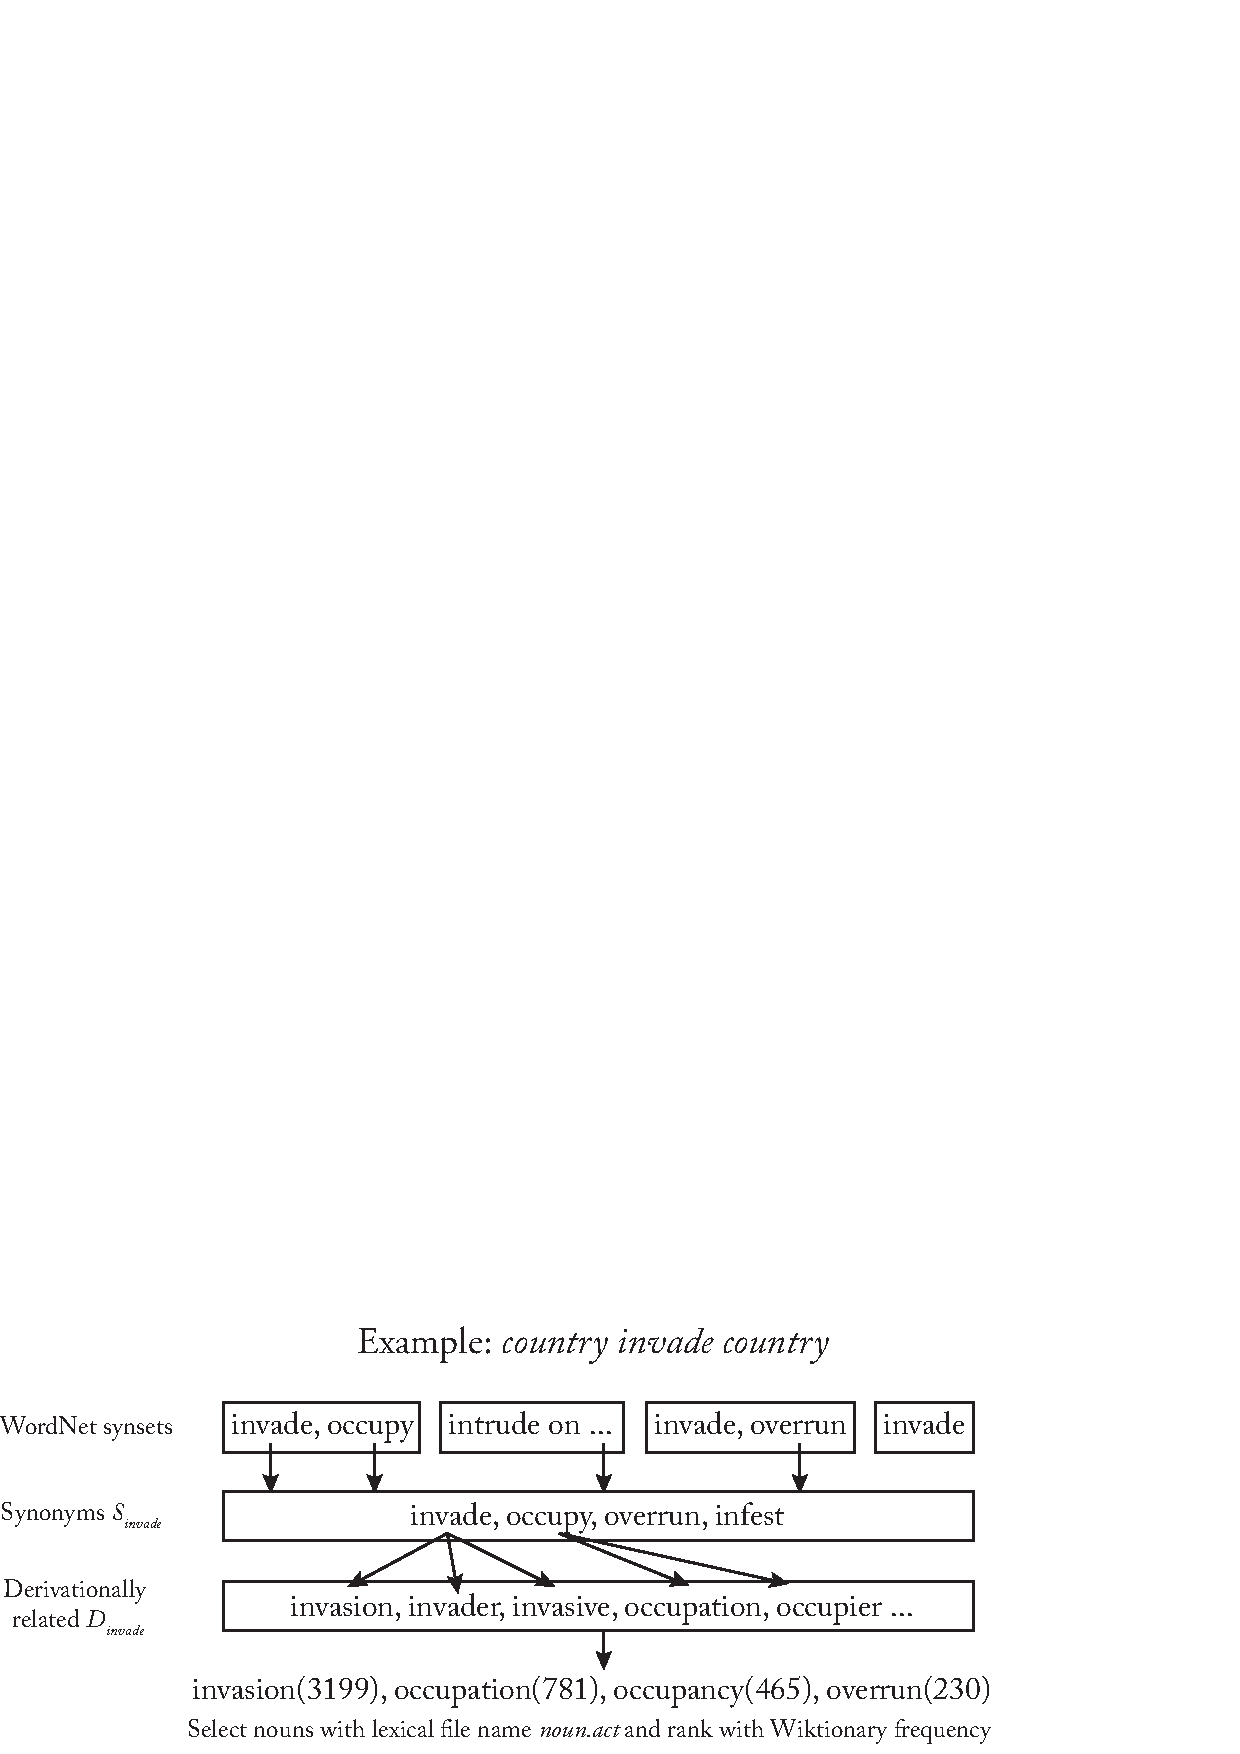
\includegraphics[width=0.95\linewidth]{img/baseline}
\caption{Baseline method}
\label{fig:baseline}
\end{figure}

\subsection{Retrieval based method}

Under the assumption that nouns in news titles are likely to be good candidates
for abstraction of action instances in the news bodies, we use a TF-IDF based retrieval method
to find the action-noun mapping.

We first build our noun dictionary $D$. Here the main sources we use are Wordnet, 
Probase and Wikitionary. In wordnet there is a field called lexical info for each token,
such as "noun.act", "noun.state". We can use these information to generate an
initial noun pool. In this stage Probase could be used in two ways, firstly it
can also be used as a pool generator. We can build the noun pool by manually designing
a small set of terms that has desired nouns as hyponyms, such terms include "activity",
"process", "event" etc. Secondly probase can also be used as a filter. We check how 
many instances a noun could have and use it as a measurement to decide whether it 
is abstract noun or concrete instances. Probase also provides the likelihood of 
the hypernym-hyponym relations which we could use too. Wikitionary is an online 
dictionary, we found a list of top 10000 popular English word there, hoping to 
solve the problem that some words in Wordnet or Probase are too obsolete.
Overall we have 4 different methods to generate the dictionary:
\begin{enumerate}
\item Use top 10000 English word as initial pool and filter by Probase
\item Use Wordnet noun iterator, combined with lexical info to build the initial pool and filter by Probase
\item Use Probase to generate the initial pool and filter by Probase
\item Use Wordnet noun iterator, combined with lexical info, no filtering
\end{enumerate}

Next we find the distribution of noun concepts in news titles, $f_n(i)$, and the distribution of action instances in news bodies, denoted as $f_{ac}(i)$ 
\begin{align*}
    f_n(i) & = \{ j |  i \in t_j \} \\
    f_{ac}(i) &= \{ k | i \in b_k \}
\end{align*}
where $t_i$ and $b_i$ are title and body of $i^{th}$ news, respectively. 

Next we use TFIDF to compute the relatedness of nouns to actions. 
\begin{equation*}
    freq(n_i, ac_j) = \bigm| \{ k | n_i \in t_k \land ac_j \in b_k \} \bigm|
\end{equation*}
\begin{equation*}
    TF(n_i, ac_j) = \begin{cases} 0 &\mbox{if freq is 0} \\
        1 + log(freq(n_i, ac_j)) &\mbox{otherwise}
    \end{cases}
\end{equation*}


\begin{equation*}
    docfreq(n_i) = \bigm| \{ k | n_i \in t_k \} \bigm|
\end{equation*}


\begin{equation*}
    IDF(n_i) = log(\frac{\text{news corpus size}}{1 + docfreq(n_i)})
\end{equation*}
